\documentclass[11pt,final]{article}%

\usepackage[square,numbers,sort]{natbib}
\usepackage{graphics}
\usepackage{amsmath,amssymb,mathrsfs}
\usepackage[usenames,dvipsnames]{color}
\usepackage[pdftex]{graphicx}
\usepackage{wrapfig}
\usepackage{url}
\usepackage{comment}
\usepackage[small,bf,up]{caption}
\renewcommand{\captionfont}{\footnotesize}
\usepackage[left=1in,right=1in,top=1in,bottom=1in]{geometry}
\usepackage{url}
% \usepackage[sf,bf,small,compact]{titlesec}
 \usepackage[sf,bf,small]{titlesec}

\titleformat{\subsection}[runin]
               {\normalfont\bfseries}
               {\thesubsection.}{.5em}{}[.]

\usepackage[mathscr]{euscript}
%% \setlength{\oddsidemargin}{0in}
%% \setlength{\evensidemargin}{0in}
%% \setlength{\textwidth}{6.5in}
%% %\setlength{\topmargin}{48pt} 
%% \setlength{\topmargin}{0pt}
%% \setlength{\headheight}{0in}
%% \setlength{\headsep}{0in}
%% \setlength{\textheight}{9in}
%% To get the default sans serif font in latex, uncomment following
%% line:
%% Note: the default sf font is much nicer than ariel/helvetica
\renewcommand*\familydefault{\sfdefault}

\def\squeeze{\parskip=0pt\itemsep=0pt}
\let\itemOld=\item
\def\item{\squeeze\itemOld}

%% \def\Heading#1{\par\bigskip\noindent\centerline{\bf\large #1}\nobreak\par}
%% \def\Subheading#1{\par\bigskip\noindent\centerline{\bf #1}\medskip}
%% \def\Subsubheading#1{\par\medskip\noindent{\bf #1.}}

%% \newcounter{sect}
%% \setcounter{sect}{0}
%% \def\Section#1{\addtocounter{sect}{1}\setcounter{subsect}{0}%
%% \par\medskip\noindent\centerline{\bf\large\thesect. #1}\nobreak\par\nobreak}

%% \newcounter{subsect}
%% \def\Subsection#1{\addtocounter{subsect}{1}%
%% \par\medskip\noindent{\bf\thesect.\thesubsect. #1.}}

% \def\Paragraph#1{\par{\bf #1.}}

% \usepackage[plainpages=false, colorlinks=true,
%   citecolor=BlueViolet, filecolor=black, linkcolor=RoyalPurple,
%   urlcolor=RoyalPurple]{hyperref}

\usepackage[plainpages=false, colorlinks=true,
  citecolor=blue, filecolor=blue, linkcolor=blue,
  urlcolor=blue]{hyperref}

\renewcommand{\baselinestretch}{0.995}

\newenvironment{nilList}
{\begin{list}{}{\partopsep=4pt plus 2pt minus 2pt
\topsep=0pt\labelwidth=10pt\labelsep=8pt\leftmargin=20pt
\rightmargin=0pt\itemsep=0pt\itemindent=-10pt}}
{\end{list}}
\def\CO2{CO$_2$}
\newcommand{\sig}{\boldsymbol\sigma}
\newcommand{\lam}{\boldsymbol\lambda}
\newcommand{\q}{\mathbf{q}}
\newcommand{\g}{\mathbf{g}}
\newcommand{\x}{\mathbf{x}}
\newcommand{\D}{\mathbf{D}}
% \newcommand{\I}{\mathbf{I}}
\newcommand{\I}{\boldsymbol{I}}
\newcommand{\K}{\mathbf{K}}
\newcommand{\Stor}{S_{\epsilon}}
% \renewcommand{\u}{\ensuremath{\mathbf{u}}}
\renewcommand{\u}{\ensuremath{\boldsymbol{u}}}
\newcommand{\s}{\boldsymbol\sigma}
% \newcommand{\f}{\ensuremath{\mathbf{f}}}
\newcommand{\f}{\ensuremath{\boldsymbol{f}}}

\newcommand{\note}[1]{\textcolor{red}{ #1}}
\newcommand{\todo}[1]{\textcolor{red}{ \bf #1}}
\newcommand{\sepu}{\vspace{10pt} \hrule \vspace{6pt}\noindent}
\newcommand{\sepl}{\vspace{6pt} \hrule \vspace{10pt}}
\newcommand{\mytilde}{\raise.17ex\hbox{$\scriptstyle\mathtt{\sim}$}}
\renewcommand{\matrix}[1] {\ensuremath{\boldsymbol{#1}}}
\renewcommand{\vec}[1] {\ensuremath{\boldsymbol{#1}}}
\newcommand{\sepu}{\vspace{10pt} \hrule \vspace{6pt}\noindent}
\newcommand{\sepl}{\vspace{6pt} \hrule \vspace{10pt}}
\renewcommand{\citep}{\cite}
\renewcommand{\citet}{\cite}

\newcommand{\zapspace}{\topsep=0pt\partopsep=0pt\itemsep=0pt\parskip=0pt}


% Title, author, date

\title{INFEWS: A Bayesian inference/prediction/control framework for sustainable groundwater management informed by geodetic data}
\author{PI: Marc A. Hesse, Co-PI's: Jingyi Chen and Omar Ghattas}

\begin{document}

\maketitle


\tableofcontents
\pagenumbering{roman}

\newpage

\pagenumbering{arabic}



\begin{center}
{\large \bf
INFEWS: A Bayesian inference/prediction/control framework for groundwater management based on the integration of geodetic data and geomechanics}
%Bayesian characterization/management of groundwater resources via
%integrated large-scale satellite geodetic data and poromechanics
%modeling}
% {\Large\bf A Bayesian computational framework for characterization
%  and management of groundwater resources via integration of
%  large-scale satellite geodetic data and poromechanics models}
\end{center}

\href{https://www.nsf.gov/funding/pgm_summ.jsp?pims_id=505241}{[Link to NSF call]}

\section{Introduction and motivation}

\subsection{The role of groundwater in the food, energy and water nexus}
% Intro GW depletion
Securing water resources for human and agricultural use while balancing the needs of the natural world is rapidly emerging as perhaps the critical issue challenging water managers at all levels of government and in the private sector. Added to concerns that already exist about water shortages and pollution, are the potential impacts of varying climate and associated extreme events such as droughts, floods, and heavy precipitation. 


% Water scarcity and food security
While all fresh water is under pressure around the globe, groundwater (GW) is of particular concern because GW extraction has tripled over the last 50 years (Figure~\ref{fig:GW Intro}\emph{a}). 
This trend is largely driven by the increase in irrigated agriculture required to feed an ever increasing world population \cite{Wada2010,Hoekstra2012}. Irrigated agriculture produces \mytilde 40\% of the global food supply and accounts for \mytilde70\% of the global freshwater consumption \cite{Siebert2010,Kummu2014}. Water for irrigation used to be mostly surface water, but today \mytilde 40\% is supplied by GW extraction \cite{Rost2008,Vorosmarty2000}. This \textbf{agricultural groundwater revolution} has fundamentally changed the role of GW in human society \cite{UNESCO2012}. In the past food production was limited by the availability of fertile land, but fresh water scarcity is projected to become the limiting factor in the near future \cite{Watkins2006,Sauer2010,Hanjra2010}. 

\begin{figure}[h]
\centering
\noindent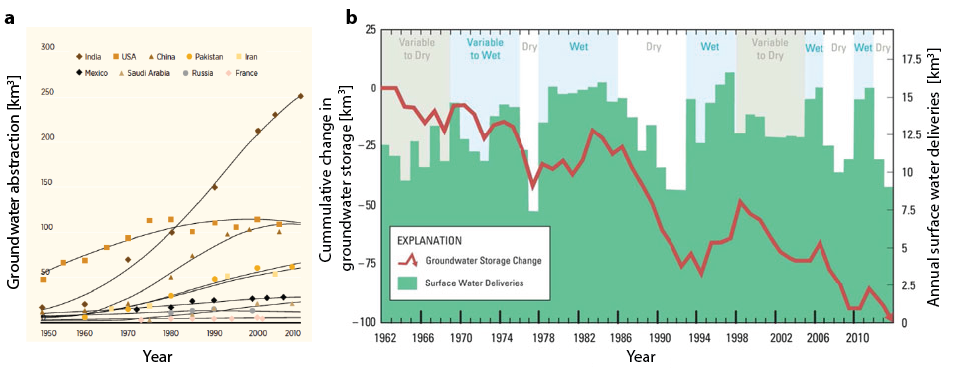
\includegraphics[width=0.8\textwidth]{Figures/Figure1.png}
\caption{\textbf{a}) Increase in groundwater extraction in the last 60 years in selected countries \cite[modified from][]{UNESCO2012}. \textbf{b})  Change in groundwater storage in the California Central Valley over the last 50 years, due to increased groundwater extraction for irrigation \cite[modified from][]{Faunt2016}}.
\label{fig:GW Intro}
\end{figure}



% A benefit of the increasing reliance of irrigation on GW is that food production is less vulnerable droughts, because aquifers storage dampens the inherent variability in precipitation.

% GW depletion
Estimates suggest that half the GW extracted for irrigation exceeds aquifer recharge and is hence unsustainable \cite{Rost2008,Vorosmarty2000}. In particular, areas with persistent water stress and large aquifer systems have increased their reliance on GW and now experience sustained GW depletion \cite{Hanasaki2008,Wada2010,Scanlon2012}. The UN Human Development Report estimates that over 1.4 billion people currently live in areas where GW depletion poses a \emph{grave threat to agricultural systems, food security and livelihoods} \cite{UNESCO2012}. The negative consequences of the GW depletion include: increased energy required for water production \cite{Scanlon2012,Narayanamoorthy2015}; irreversible aquifer compaction and loss of GW storage (Figure~\ref{fig:GW Intro}\emph{b}); degradation of GW groundwater dependent ecosystems and loss of ecosystem services \cite{Klove2014,Doody2017}; flooding and saltwater intrusion and coastal areas \cite{Erban2014b,Alfarrah2018}.  The first two are most relevant to this proposal.

% Groundwater depletion and energy for food production
\emph{The relationship between water and energy is reciprocal} \cite{UNESCO2012}. Groundwater extraction accounts for \mytilde8\% of energy production globally and up to 40\% of the energy produced in developing countries \cite{WorldEconomicForum2011}.
As GW depletion progresses the energy intensity of irrigation increases, because the deeper wells have to be drilled and GW has to be raised from grater depth. In extreme cases, failing GW supplies have to be supplemented by imports of surface water transported over large distances. This increases the cost of irrigation will have adverse effects on both farmers and consumers, in particular in the developing world \cite{Narayanamoorthy2015}.

% GW storage to limit risk
The permanent loss of GW storage in depleted aquifers also increases the vulnerability of water supplies and food production to climate change \cite{Taylor2013}. In many arid regions climate change is expected to result in reduced and more variable rainfall. Due to the relatively large volumes of water stored underground, most aquifers have a considerable buffer capacity, which keeps their water available for withdrawal even during very long periods without rainfall  \cite{UNESCO2012}. Maintaining GW storage by preventing overpumping therefore plays a crucial role in our adaptation to climate change.

\subsection{Role of GW resource management at the Food-Energy-Water (FEW) Nexus}
% This is Really what INFEWS wants to fund!
The increasing extraction of GW for irrigation around the globe is a key element of the FEW-nexus that determines global food security, requires significant fraction of global energy and plays a crucial role in climate change adaptation.  The UN Human Development Report therefore concludes that careful GW management \emph{can make a significant contribution to meeting the demand for water in the future and to adapting to climate change} \cite{UNESCO2012}. The report defines \emph{water management} as managing the resource, managing water services, and managing the trade-offs needed to balance supply and demand. 

In the twenty-first century, water management has moved from hard solutions favoring large infrastructure projects to a range of softer measures based on institutional reform, incentives and behavioural change that aims to increase resilience and decrease vulnerability \cite{Wolff2002,Brooks2011}. In this soft path to water management, \textbf{the role of water managers is to inform the decisions taken by others} and to provide forecasting and modelling to facilitate more accurate risk assessment \cite{UNESCO2012}. In herent in the soft path is  an \textbf{adaptive management} approach where improvements are made gradually in a monitoring and assessment cycle.

Here we focus on \textbf{water resource management}, which includes water allocation, assessment and pollution control; the protection of water-related ecosystems and water quality; redistribution and storage of these resources; and groundwater recharge. This proposal is focused on GW resource management, because GW is till the least understood component of the hydrologic cycle \cite{Re2015} and introduces significant uncertainty and risk into any integrated water management strategy. The challenge of GW resource management is highlighted in a recent expert survey, which concluded that \emph{solutions for the monitoring and management ... of .. withdrawals from aquifers to ensure they do not exceed the mean recharge rates} are unlikely to occur in the short term. 

% Water management is underpinned by levels of uncertainty. Adapting to these uncertainties and developing strategies that mitigate against emerging risks makes water management policies, institutions and regulations more resilient. Adaptive water management extends to IWRM by focusing on a more flexible management process to address uncertainty.

% 5.1.2 Integrated water resources management IWRM is defined as a process that ‘promotes the coor- dinated development and management of water, land and related resources in order to maximize the result- ant economic and social welfare in an equitable man- ner without compromising the sustainability of vital ecosystems’ (GWP-TAC, 2000, p. 22).


\subsection{Climate change, increasing uncertainty and adaptive GW resource management}\label{sec:adaptive}
The dominant natural sources of uncertainty in GW resource management stem from the sparse sampling of aquifers and increasing climate variability and change. The confluence of these two factors introduces increasing uncertainty that poses unique challenges for decision-makers and must be addressed by risk management \cite{Shaw2010}. It is therefore essential that any GW resource management strategy acknowledges these uncertainties and integrates them into ... \note{say something smart and to the point!} 

The dominant uncertainty in the predictions of any GW model is the insufficient characterization of the aquifer properties \cite{Eaton2006,Bohling2010,Oliver2011}. These properties, such as its \textbf{permeability} which governs the flow of GW and \textbf{specific storage} which determine the volume of GW, can change by several orders of magnitude and display lateral variability on all scales. In principle, the uncertainty in these parameters could be quantified with Bayesian inference, if sufficiently rich data-set were available \cite{Carrera1986a,Carrera1986b,McLaughlin1996}. However, classic aquifer characterization based on sparse measurements at wells has often not been sufficient to significantly reduce the uncertainty in model predictions \cite{Bohling2010}. This uncertainty is exacerbated by increasing climate variability due to climate change. As water scarcity increases GW depletion the aquifers are driven to new states that are not informed by past data and experience. 
It will therefore \textbf{no longer possible to use today’s science, based on yesterday’s experience, to predict the needs of the future} \cite{Turton2007}. \note{(I know it sounds corny !)}

Hence there is a need to improve GW monitoring and integrate new data into GW models to reduce the uncertainty in predictions and hence to facilitate decision-making. The need for adaptive management requires that new data is continuously integrated into GW models to update projections of resource allocation and the associated uncertainties. Optimally, the data also provide a way to track the effect of management changes on the GW system to assess their success.

% integration between data acquisition, assimilation into models and 
% for com- plex data, hard-wired into feedback loops, specifically for managing the incremental changes needed in the various systems including the means of tracking those changes (Stakhiv and Pietrowsky, 2009).

% \subsection{Adpative }

% One of the most direct ways of reducing uncertainty is to generate new knowledge or understanding of conditions governing water availability and quality in the present and in the future. Data collection, analytical capacity and predictive ability are all required to reduce uncertainty and therefore to facilitate decision making about allocations, uses, mobilization and treatment. While the risk to water is not reduced, it is better understood.

% Decision-making that embraces uncertainty and risk

% There is a need for increasingly sophisticated monitor- ing systems to source and integrate the necessary data. This adds additional stresses to the overall decision- making process. 

% Traditionally, analysis of past climate coupled with stochastic analysis has provided a fairly reliable basis for examining the water cycle with its hydrological extremes. Historical.

% Any study of strategy, planning, design, operation and management of water resources systems must take as its basis variability of quantity and quality in water sources and supply systems. 

\subsection{Opportunities in geodetic aquifer characterization}
Fortunately, remote sensing and geodetic measurements have begun to provide a wealth of new, spatially-distributed time-series data that promise to significantly improve the characterization of the subsurface beyond what can be provided by well data alone and have been identified as the most valuable groundwater monitoring technologies. These include total water storage change from the Gravity Recovery and Climate Experiment (GRACE) and the GRACE Follow-on (GRACE-FO) mission. In particular, surface deformation data derived from interferometric synthetic aperture radar (InSAR) (1992-present) can be used for characterizing groundwater levels and storage properties in confined aquifers, the critical metric needed for effective groundwater management. While spaceborne Earth-observing missions have provided large amounts of data that can be used to study freshwater resources, these data have been greatly under-utilized in operational water management practices. A grand challenge we need to address today is how to assimilate satellite and in-situ data into quantitative, predictive and computational groundwater models to better assist decision making.

Galloway and Hoffmann [2007] \cite{Galloway2006a} show that satellite InSAR has (1) allowed the identification of the structural and stratigraphic boundaries to fluid flow and deformation, (2) placed constraints on the magnitudes of subsurface material properties and their heterogeneity, and (3) allowed calibration of numerical models of subsurface flow and the associated deformation.

% In recent years, remote sensing and geodetic measurements have begun to provide a wealth of new, spatially-distributed time-series data on surface deformation in response to fluid injection (Figure \ref{fig:InSAR}). These observations promise to significantly improve
% the characterization of the subsurface beyond what can be provided by
% well data alone and have been identified as the most valuable monitoring technology for large scale GCS \cite{Mathieson2010}.

% \subsection{Challenges and opportunities in aquifer characterization}

% However, GW is still the least understood component of the hydrologic cycle \cite{Re2015} and introduces significant uncertainty and risk into any water management strategy. The uncertainty in any prediction of GW availability is largely due to the geological complexity of aquifers.  This leads to large variations in aquifer properties that are only sparsely sampled at wells. The predictive power of GW models is therefore often too limited to allow model-predictive decision making.

\subsection{Aim of this proposal}
Driven  by these recent developments, we propose to develop a \textbf{Bayesian poromechanics-based inversion/control framework for GW resource management}. This framework takes into account uncertainties at every stage and aims to reduce uncertainty in predictions though the \textbf{assimilation geodetic observations}.  Using this approach we aim to produce actionable forecasts of head levels and projections of sustainable well extraction rates with a lead time of 30 to 180 days. Continuous and automatic assimilation of new data will update the forecast and allow the deployment of adaptive management strategies. 

Achieving this requires the integration of the following three components
\begin{enumerate}
    \item Automated processing of InSAR data to produce estimates of land surface elevations.
    \item Integrate this satellite and well data with coupled poromechanics models of subsurface deformation and flow by solving the {\bf inverse problem} for unknown subsurface properties and aquifer recharge.
    \item Use the resulting inferred poromechanics models to design {\bf optimal control} strategies for GW extraction that maximize the water availability while preventing aquifer compaction. 
\end{enumerate}

To test if the geodetic data is sufficiently rich and poromechanic models are sufficiently predictive to warrant model-predictive decision making this framework will be applied to a testbed provided by GW dependent irrigation in the San Louis Valley (SLV), CO. We have chose this example, because many of the challenges faced in the SLV are symptomatic for the global challenge of sustainable GW management.


\section{Background Significance, and Outstanding Challenges}
First we describe the application where the proposed framework will be tested in \S\,\ref{sec:SLV}, because this sets the objective of the inversion/control problem that will subsequently be addressed. This is followed by brief outlines to poromechanic forward model in \S\,\ref{sec:poromech}, the Bayesian inverse model in \S\,\ref{sec:bayesian}, and optimal control under uncertainty \S\,\ref{sec:control}.
\note{something about the outstanding challenge}


\subsection{Testbed: Irrigation in the San Luis Valley, CO }\label{sec:SLV}
The San Luis Valley (SLV) is located in the northern half of the Rio Grande Basin, bounded to the east by the Sangre De Cristo Range and to the west by the San Juan Mountains as shown in Figure \ref{fig:SLV} \citep{SLV_report}. The valley fill consists of interbedded deposits of sand, clay, gravel, and some layers of volcanic rocks, underlain by volcanic basement. The Rio Grande flows through the valley but does not drain the northern portion, which is a closed drainage basin. The southwestern portion of the Valley contains the Conejos and Alamosa River Valleys, which are adjacent to a series of mesas and eroded hills called San Luis Hills.

\begin{figure}
\noindent\includegraphics[width=1\textwidth]{Figures/Figure2.pdf}
\caption{\textbf{a}) Geographic boundaries (defined by the white lines) and the outline of the San Luis Valley (defined by the purple line). The red line is the state boundary between Colorado and New Mexico. The top left panel illustrates the location of the San Luis Valley in the state of Colorado. Black lines indicate locations of two coss-sections in panels \emph{c} and \emph{d}. \emph{b}) Fence diagram showing the major geological units of the basin fill. \emph{c} Cross-section along the valley between A and A' in panel \emph{a}. \textbf{d}) Cross-section across the deepest part of the valley between E and E' in panel \emph{a}.}
\label{fig:SLV}
\end{figure}

Groundwater pumping occurs mainly in the Closed Basin and the Conejos and Alamosa River Valleys, and is essential for supporting the vibrant agricultural economy of this high-altitude desert-climate valley. Over much of the valley, the top 50 to 130 feet of sediments constitutes an upper unconfined aquifer overlying a larger confined aquifer. The unconfined aquifer is the principal source of groundwater in the area, with considerable interest in increased withdrawal of water from the confined aquifer.  \textcolor{red}{The Colorado legislature has directed that in order to continue use of the confined aquifer the SLV managers must maintain head levels in the aquifer at 1978-2000 levels.} The Rio Grande Decision Support System (RGDSS) is a MODFLOW model of the SLV that is used to predict head levels in the confined aquifer  \citep{RGDSS}.  Head data over the active area of water use are sparse in 1978, but grow more robust to the present although the monitoring data points are unequally distributed. The lack of historical and well-distributed head data impacts the accuracy of the modeling.  There is great interest in the ability to assimilate satellite and in-situ data into quantitative, predictive and computational groundwater flow models to better assist decision making.

We propose to develop a prototype system for application in the San Luis Valley of Colorado. Our modeling approach builds a predictive model through the analysis of >20 years (1992-present) of in-situ and satellite data to determine the spatial and temporal links between hydraulic head and other principle components of the basin-scale water cycle - precipitation, run-off, evapotranspiration, surface water, soil moisture, and groundwater pumping; the predictive model is continually updated with the addition of newly acquired data. Because we cannot measure head directly except at sparse well locations, we will use recently-developed InSAR methods deriving subsidence over time to obtain temporally and spatially dense head estimates.  Once calibrated with local well-based measurements, these observations will be integrated using the predictive model to predict future head levels. In developing the predictive model to forecast head, the study area will be expanded beyond the SLV to the basin headwaters in the San Juan and Sangre De Christo mountains. We aim to discover a reliable predictive link between snow accumulation and melt and head changes in the confined aquifer.  While evidence suggests that the snowpack at lower elevations is the primary source of recharge to the confined aquifer, there is not a solid quantitative basis for making reliable predictions of head changes in the aquifer.  Such a predictive capability would be extremely valuable and would allow Colorado water managers to take proactive measures if low heads were predicted.  For example, fields could be fallowed, or water from the Rio Grande could be used to recharge selected areas of the aquifer.

% Here is a little more infomoation of the SLV groundwater aquifers, some cross-sections of the hydrogeologic layers acress the SLV are also available
Groundwater pumping occurs mainly in the Closed Basin and the Conejos and Alamosa River Valleys, and is essential for supporting the vibrant agricultural economy of this high-altitude desert-climate valley. Currently, the Rio Grand Decision Support System (RGDSS), which includes a hydrogeologic database and a MODFLOW finite-difference groundwater flow model, is being used to quantitatively evaluate and manage the groundwater resources in the SLV. The conceptual RGDSS hydrogeologic model of the SLV consists of five distinct hydrogeologic layers \citep{RGDSS}. Here we summarize the available hydrogeologic information of the SLV aquifer as described in \textcolor{red}{Judge Kuenhold's decision in the confined aquifer case \citep{Rules}}. Over much of the valley, the top 15 to 40 meters (50 to 130 feet) of the sediment thickness (layer 1) constitutes an upper unconfined aquifer. A confining layer known as an aquitard (layer 2) progresses from solid clay near the central axis of the SLV (generally along Hwy 17 from Moffat to Alamosa) to clay lenses interspersed with sands. The sand to clay ratio generally increases outward from the central axis and the aquitard thickness diminishes at the edge of the SLV. Layers 3-5 are the confined aquifer system. Layer 3 is generally interpreted to be the most productive portion of the confined aquifer system. In the northern portion of the SLV, layer 3 contains mainly sand, although clay layers do appear. In the southern portion of the SLV, layer 3 is composed of the Hinsdale and Servilleta Basalt and sand. Layer 4 is a mix of sand and gravel with as much as 50 percent clay in most areas of the SLV. The confined aquifer becomes more clay rich with depth and layer 5 is generally not considered to be a productive aquifer due to its low hydraulic conductivity.

\begin{figure}
\noindent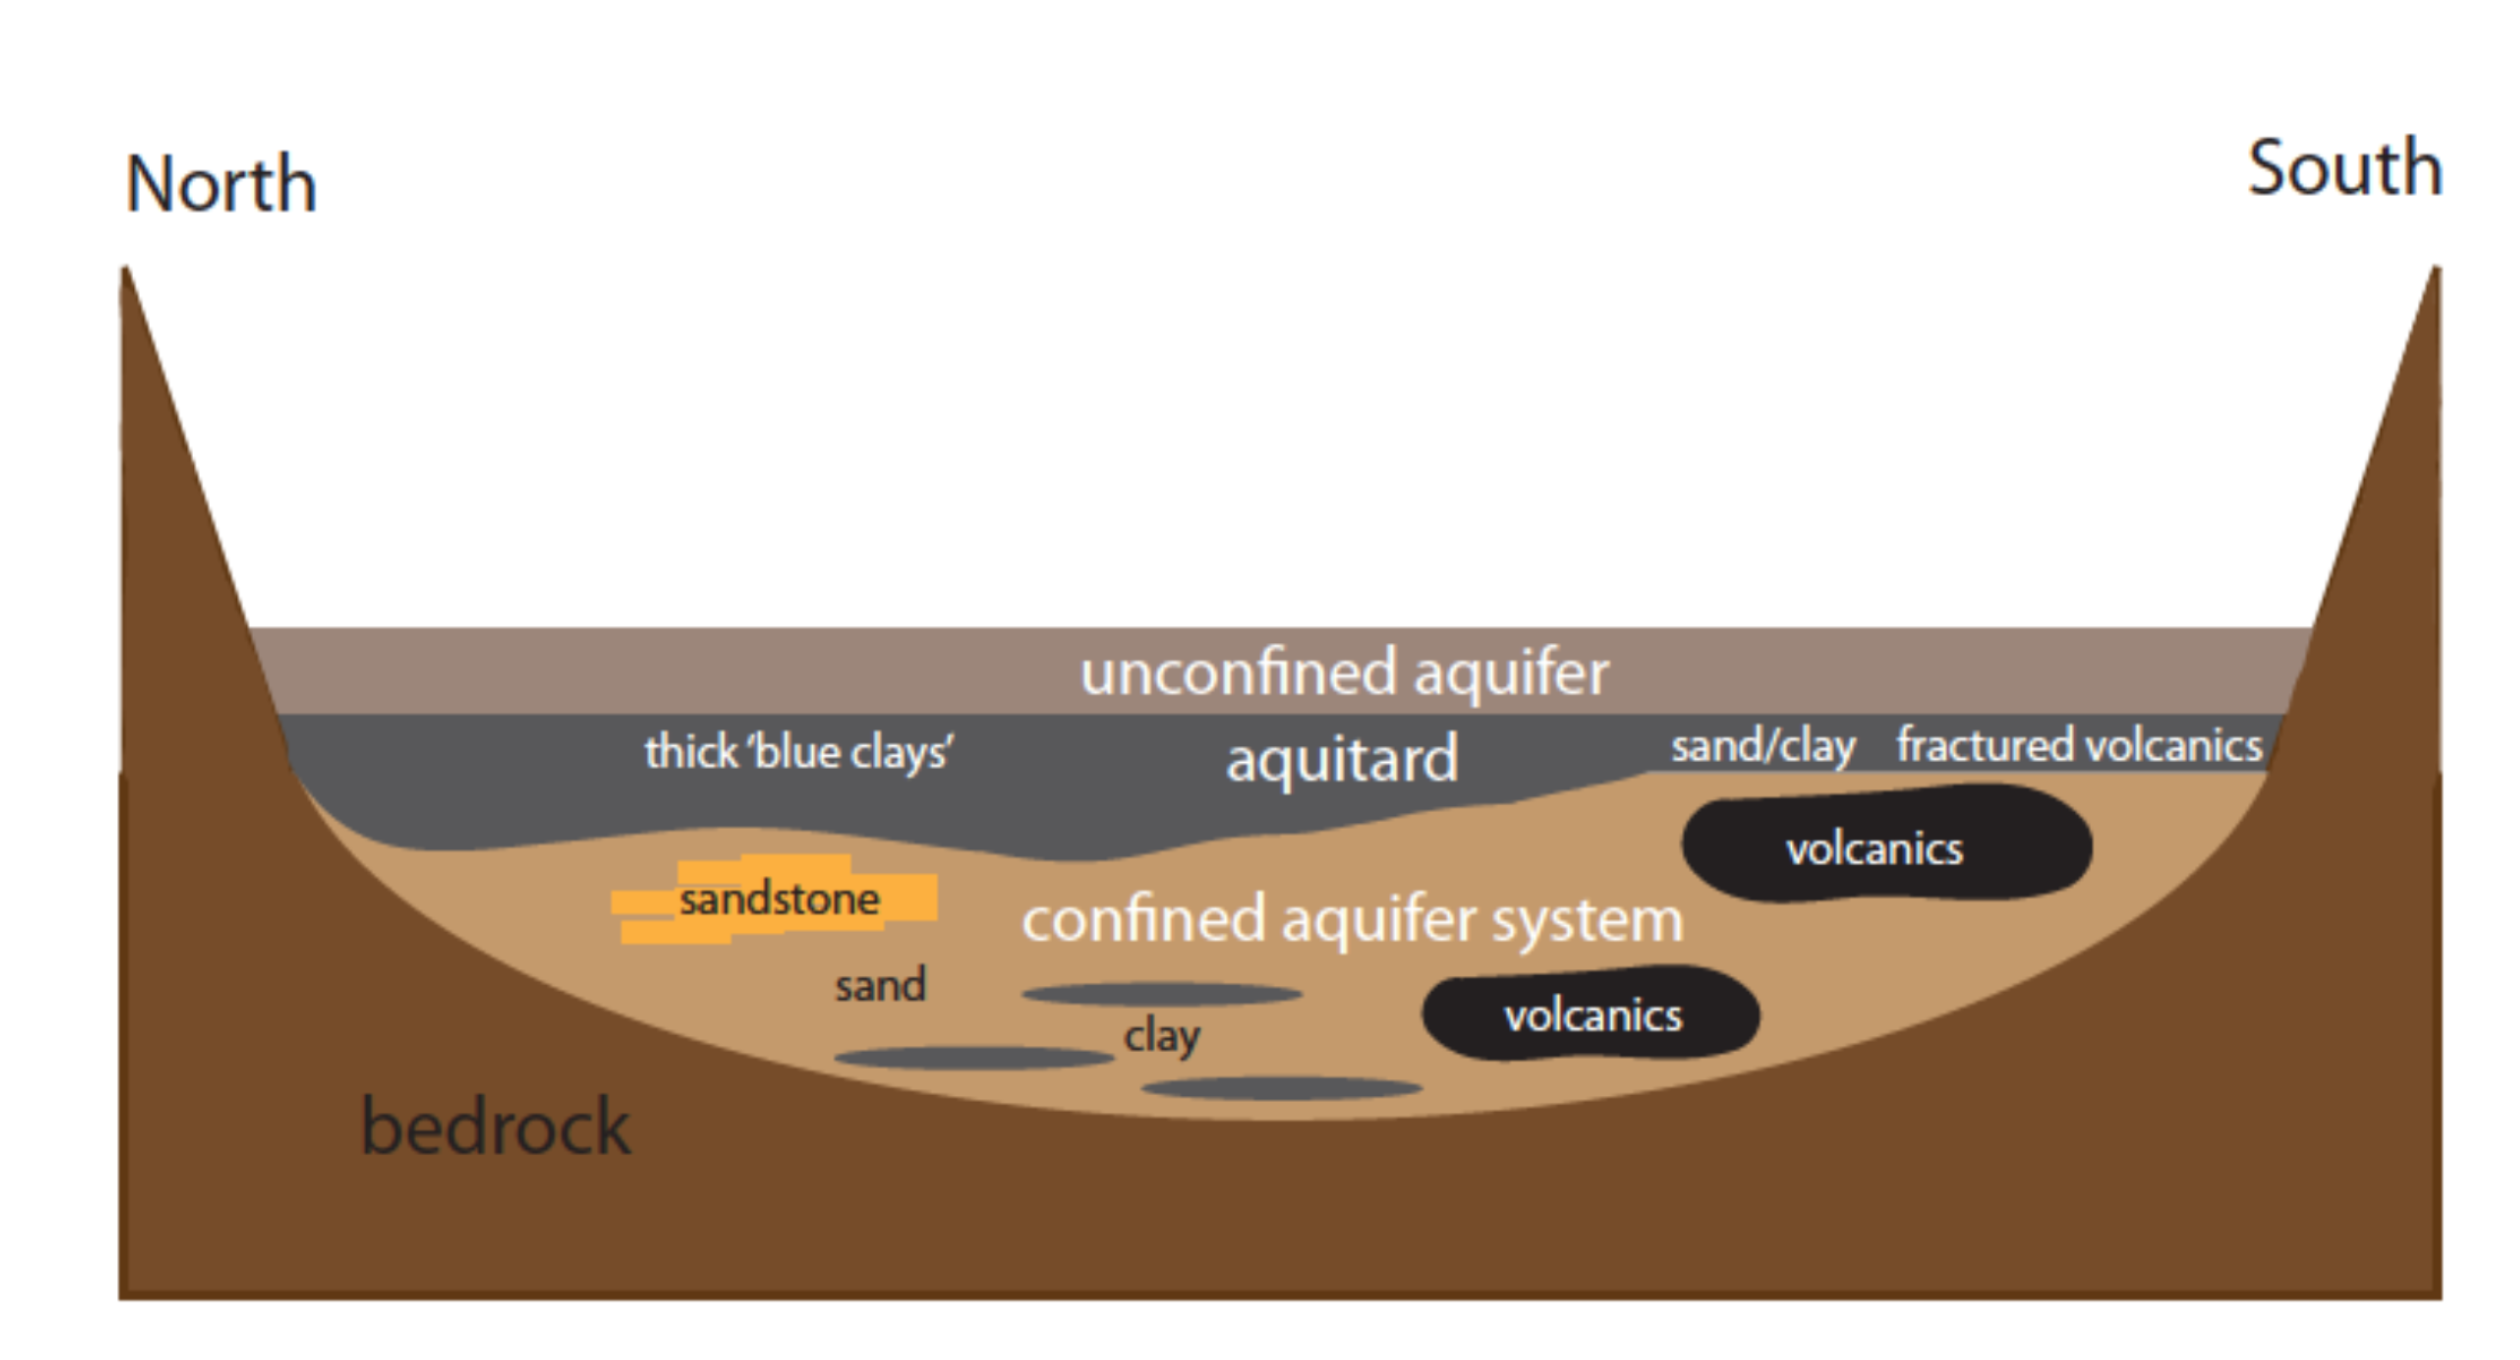
\includegraphics[width=0.9\textwidth]{Figures/SLVaquifers.png}
\caption{A schematic showing the variable geology of the hydrogeologic layers from north to south in the San Luis Valley (J. Reeeves, 2013).}
\label{fig:slv-aquifers}
\end{figure}


\subsubsection{Water Balance Model}
Understanding the availability of freshwater resources requires measurement of key components in the freshwater cycle shown in Figure \ref{fig:watercycle}. Here we consider the surface water and boundary layer as a single element, denoted surface water. The net freshwater fluxes can be approximated by the following equation:
\begin{align}
\Delta SM +\Delta S^s +\Delta S^u + \Delta S^c = P-ET-Q
\label{eq:waterBalance}  
\end{align}
where $P$ is precipitation, $ET$ is evapotranspiration, $Q$ is the river runoff. $\Delta SM$ is the change in soil moisture, $\Delta S^s$ is the change in surface water storage in rivers and lakes, $\Delta S^u$ is the change in unconfined aquifer storage, and $\Delta S^c$  is the change in confined aquifer storage.

\begin{figure}
\noindent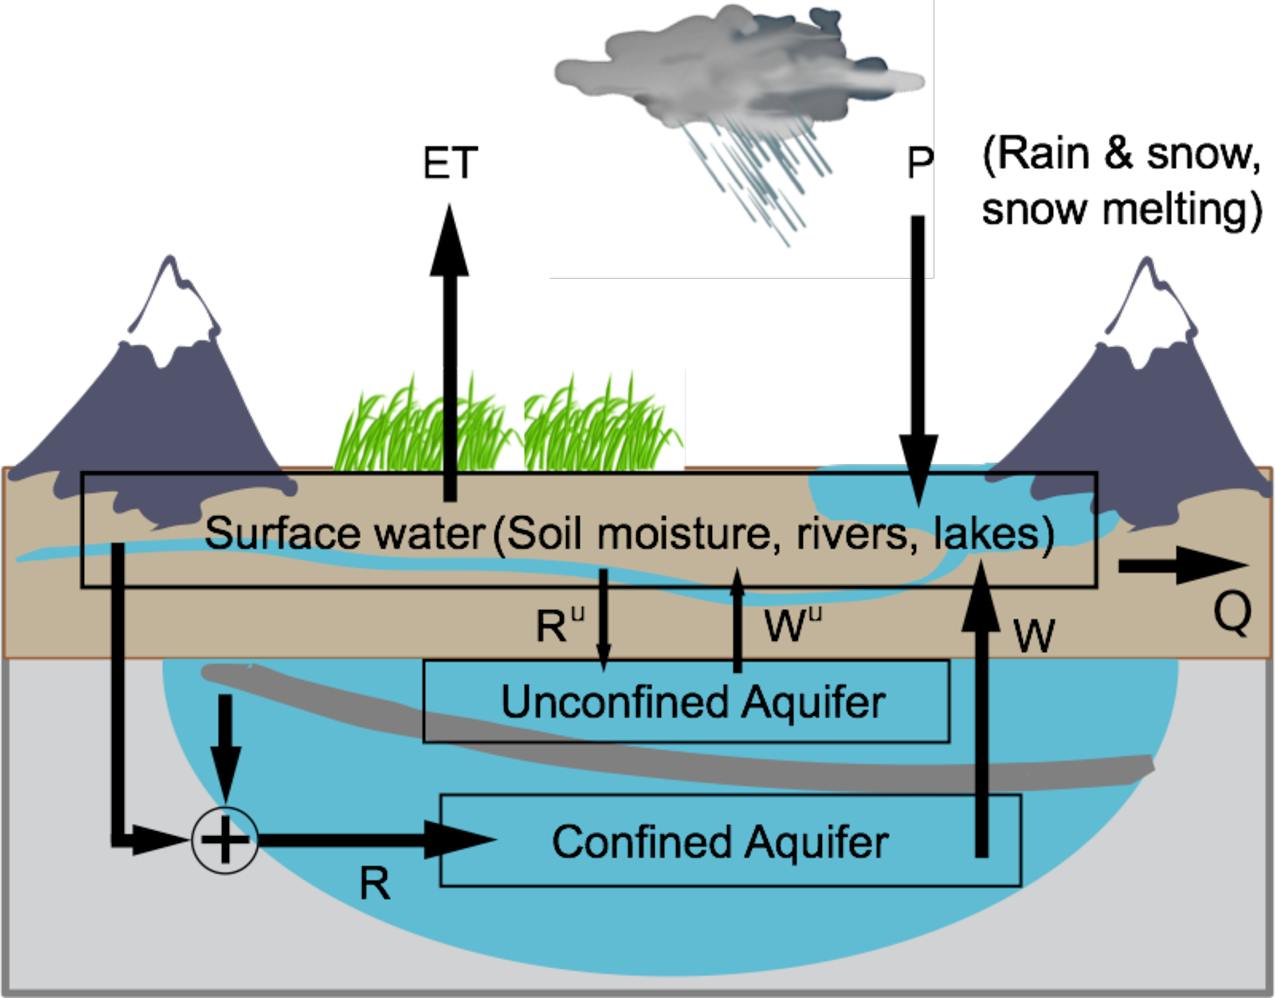
\includegraphics[width=0.6\textwidth]{Figures/watercycle.pdf}
\caption{Water balance model. In this model surface water and soil moisture are combined into the “surface water” box.  The terms marked in blue are the key elements of the water balance equation; their interrelationships are discussed in Equation \ref{eq:waterBalance}.}
\label{fig:watercycle}
\end{figure}

The change in confined aquifer storage $\Delta S^c$ can be further expressed as:
\begin{align}
\Delta S^c = R - W
\label{eq:confinedStorage}  
\end{align}
where $W$ is the withdrawal from the confined aquifer and R is the recharge. Given a \textcolor{red}{minimum safe storage level for the confined aquifer} $\Delta S^{C-min}$, we can manage the storage of the confined aquifer by scheduling withdrawals such that withdrawal ceases when (in our convention withdrawal leads to negative $\Delta S^c$):
\begin{align}
\Delta S^c = P-ET-Q-\Delta SM - \Delta S^s - \Delta S^u = R-W < \Delta S^{C-min}
\label{eq:safelimit}  
\end{align}
Note that $\Delta S^c$  can be considered as a source term describing the forcing of water into the confined aquifer.  We therefore introduce an additional notation to emphasize its role as a source and its explicit dependence on both space and time:
\begin{align}
U(x;t) = \Delta S^c
\label{eq:force}  
\end{align}

% \subsection{Surface deformation due to Subsurface Hydrology}
% Anthropogenic land subsidence associated with withdrawal of fluids from the subsurface due to groundwater extraction and the production of hydrocarbons has been recognized for decades \citep{Poland1969}, for recent reviews, see Gambolati et al. \cite{Gambolati2005} and Galloway and Burbey \cite{Galloway2011a}. While subsidence is generally slow, the rates of the induced land subsidence can locally reach several centimeters per year and cumulative subsidence over several decades of fluid withdrawal can reach tens of meters in severe cases, such as the rapid compaction of lacustrine sediments beneath Mexico City [Ortega-Guerrero et al., 2009; Osmanoglu et al., 2011]. Anthropogenic land uplift is associated with the injection of fluids for enhanced oil production, natural gas and carbon dioxide storage, aquifer storage and recharge, and the injection of industrial waste [Teatini et al., 2011]. Cumulative land uplift due to fluid injection is on the order of several centimeters and is therefore often not recognized, unless it is systematically monitored. In both cases—subsidence and land uplift—the lateral extent of the deformation is large and we will refer to it below as (regional) surface deformation.

% \subsection{Geodetic surface deformation measurements}
% The systematic measurement and monitoring of the evolution of regional surface deformation is challenging due to the large spatial scales, the need for stable geodetic reference marks, and repeated surveys \citep{Galloway2011a}. In the last decades, ground-based geodetic surveys have been complemented by the global positioning system (GPS) and by remotely sensed geodetic surveys such as airborne light detection and ranging (LiDAR) as well as satellite-based differential interferometric synthetic aperture radar (InSAR) \citep{Galloway1998,Burgmann2000} and Persistent/Permanent Scatterer interferometry (PS-InSAR) \citep{Ferretti2001}. Satellite InSAR and PS-InSAR are ideally suited for the measurement of surface deformation associated with fluid injection or extraction, because it allows the mapping of areas as large as 10,000 km2 while a single picture element (pixel) may have a resolution of up to 5 m [Hanssen, 2001].Within a pixel, InSAR can detect vertical displacements on the order of 10 mm or less and PS-InSAR may allow the detection of displacements with an accuracy of 1–2 mm \citep{Ferretti2001}. In the last decade, these techniques have been used to generate detailed time series images of regional surface deformation that have greatly advanced our understanding of the sub- surface. 

% \subsection{Aquifer characterization}\label{sec:aquifer characterization}
% All properties of the subsurface are spatially vari-
% able and often anisotropic, but the permeability often has the strongest spatial variation and usually dominates the flow field. The characterization of the permeability field is therefore key to successful prediction of flow and trans- port processes in the subsurface. In practice, the information available for this characterization is sparse and the uncertainty in the estimated properties is large. To make the inverse problem well posed and to characterize the uncer- tainty of the estimate, hydrological inversions use Bayesian inference to incorporate prior information [Carrera and Neuman, 1986; McLaughlin and Townley, 1996; Woodbury and Ulrych, 2000; Castagna and Bellin, 2009; Rubin et al., 2010]. [5] The characterization of aquifers based purely on hydraulic data, briefly reviewed in section 1.2.1, often has very large uncertainties. The reduction of this uncertainty is the motivation to include additional data into the characteri- zation and has led to increased interest in hydrogeophysical methods and joint inversions of hydraulic and geophysical data. The poroelastic inversion discussed here is a spe- cial case of hydrogeophysical inversion that aims to add deformation measurements to hydraulic data. Section 1.2.2 summarizes previous work on poroelastic inversion.
% 1.2.1.



\subsection{Poromechanics forward model}\label{sec:poromech}

To describe the coupling of subsurface flow with the deformation of the pore skeleton, we require a poromechanics model. Biot's linear quasi-static poroelasticity equations  \citet{Biot1941}
generally provide a good match with field observations. The PDEs for the evolution of the fluid pressure $p=p(x,t)$ and the solid displacement $\u=\u(x,t)$ are given by (see \citet{Wang2000})
\begin{subequations}\label{eq:Biot strong}
\begin{alignat}{2}
\left(\Stor p+\alpha\nabla\cdot\u\right)_t-\nabla\cdot\left(\kappa/\mu\, \nabla p\right)&=f &&  \text{ in }\Omega\times (0,T), \label{eq:mass}\\
 -\nabla\cdot\left(\s(\u) -\alpha p\I\right)&=\f && \text{ in }\Omega\times (0,T), \label{eq:mom}
\end{alignat}
\end{subequations}
where $\Omega$ is the modeled domain and $(0,T)$ denotes the interval for the time evolution.  The poroelasticity PDE system \eqref{eq:Biot strong} is completed by suitable initial and boundary
conditions.  Equation \eqref{eq:mass} describes the conservation of fluid mass, where $\Stor$ is the specific storage at constant strain, $\kappa(x)$ is the permeability, $\mu$ is the fluid viscosity, and
$f(x,t)$ is a source or sink term due to fluid injection or production at wells.  Equation \eqref{eq:mom} reflects total momentum conservation in the porous medium, where $\s$ is the elastic stress
tensor, $\alpha$ the Biot-Willis parameter, and $\f(x,t)$ the volumetric body force.  The elastic stress
tensor in terms of the solid displacements is given by
\begin{alignat*}{1}
 \s(\u)&=G\left(\nabla\u+\nabla^{T}\u\right)+\frac{2G\nu}{1-2\nu}\left(\nabla\cdot\u\right)\I, %\label{eq:sig'}
\end{alignat*}
where $G$ and $\nu$ are the drained shear modulus and Poisson's ratio, respectively.  

The governing equations contain six independent parameter fields. There are four mechanical parameters $\Stor$, $\alpha$, $G$ \& $\nu$ and two hydraulic parameters $\kappa$ \& $\mu$. In shallow groundwater applications the water viscosity $\mu$ can be assumed to be constant and most geological application Poisson's ratio is typically set to $\nu = 0.25$. The remaining four fields are unknown and spatially variable. The specific storage $\Stor$ and permeability $\kappa$ determine the aquifer response to pumping and recharge and are hence of greatest interest. The Biot-Willis parameter, $\alpha$, and drained shear modulus, $G$, determine the deformation that results from groundwater flow and hence the surface deformation that can be observed by InSAR.

For the testbed outlined in \S\ref{sec:SLV} the annual recharge of the aquifer due to snow melt in the spring is essential for the cyclical behavior shown in Figure \note{X}. In the model this recharge is represents by a temporally and spatially varying flux, $q_r$, applied to the lateral boundary, $\partial\Omega_l$, of the aquifer
\begin{align}
    \mathbf{q}\cdot\hat{\mathbf{n}} = q_r(s,t)\quad \mathbf{x} \in \partial\Omega_l \times (0,\,T),
\end{align}
where $s$ is a arc-length coordinate along the boundary and $\mathbf{q}$ is the volumetric flux from Darcy's law.


%Characterizing the permeability field is key to successful prediction of pore pressure perturbations and induced seismicity. Because of the multiple orders of magnitude variation in the permeability, the wide range of spatial and time scales exhibited, and the complex subsurface geometries, the design of efficient discretization methods as well as parallel mesh adaptivity and scalable solvers has proved elusive. In \S\ref{sec:solver} and \S\ref{sec:amr}, we describe proposed work aimed at overcoming these challenges.

\subsection{Bayesian inversion}\label{sec:bayesian}

In the Bayesian approach, we state the inverse problem as a problem of
\emph{statistical inference} over the space of uncertain parameters,
which are to be inferred from the data and a physics-based model.
The resulting solution to the statistical inverse problem is a
posterior distribution that assigns to any candidate set of parameter
fields our belief (expressed as a probability) that a member of this
candidate set is the ``true'' parameter field that gave rise to the
observed data.
%
When discretized, this  infinite-dimensional inverse problem  gives
rise naturally to a large-scale problem of inference over the discrete
parameters
% space
$\vec{x} \in \mathbb R^n$, corresponding to degrees of
freedom in the parameter field mesh.
%  While the presentation in
%this paper is limited to the finite dimensional approximation to
%the infinite dimensional measure, the discretization process is
%performed rigorously following \cite{Stuart10,
%  Bui-ThanhGhattasMartinEtAl12}, and the numerical evidence indicates
%that we converge to the correct infinite dimensional distribution.

%% candidate parameters $\vec{x}$ a value $\pi_{\text{post}}(\vec{x})$,
%% which reflects our degree of confidence that the parameters $\vec{x}$
%% might be the true values that gave rise to the data.

The posterior probability distribution combines the prior pdf
$\pi_{\text{prior}}(\vec{x})$ over the parameter space, which encodes
any knowledge or assumptions about the parameter space that we may
wish to impose before the data are considered, with a likelihood pdf
$\pi_{\text{like}}(\vec{y}_{\text{obs}}|\vec{x})$, which explicitly
represents the probability that a given set of parameters $\vec{x}$
might give rise to the observed data $\vec{y}_{\text{obs}} \in
\mathbb{R}^m$.  Bayes' Theorem then explicitly computes the posterior
pdf as
% \begin{align*}
$ \pi_{\text{post}}(\vec{x} | \vec{y}_{\text{obs}}) \propto
\pi_{\text{prior}}(\vec{x}) \pi_{\text{like}}(\vec{y}_{\text{obs}} | \vec{x})$.
% \end{align*}
%% We choose the prior distribution to be Gaussian, with a covariance
%% operator defined by
%% % twice its action as the solution of an elliptic PDE.
%% % OG: I found the preceding line confusing.
%% the square of the inverse of an elliptic PDE operator.
%% This choice yields several benefits.  First, it enables
%% % storage
%% % OG: we don't really store the covariance (i.e. the *inverse* of the
%% % laplacian)
%% implicit representation of the prior covariance operator as (the
%% inverse of) a sparse operator, as opposed to traditional approaches
%% that either store a dense covariance matrix or its approximation by
%% principle vectors.  Second, since the covariance operator is never
%% needed explicitly---only its action on a vector is required--- we are
%% able to capitalize on fast $O(n)$ parallel elliptic solvers (in this
%% paper, algebraic multigrid) to form this action via two elliptic
%% solves. Third, the action of the symmetric square root factorization
%% of the prior covariance is available explicitly (via one elliptic solve
%% instead of two). Finally, this choice of covariance is useful for
%% technical reasons, as it % provides sufficient conditions to
%% guarantees
%% that samples from the prior distribution will be continuous.
%% % OG: should we say the following?
%% % and thus the inverse problem is well-posed
%
For many problems it is reasonable to choose the prior distribution to
be Gaussian. If the parameters are coefficients corresponding to a
discretization of a field, the prior covariance operator usually
imposes smoothness on the parameters, which is also important to state a
physically meaningful infinite-dimensional Bayesian inverse problem
\cite{Stuart10,Bui-ThanhGhattasMartinEtAl13}.
%% The difference between the observables predicted by the
%% model and the actual observations $ \vec{y}_{\text{obs}}$ is due to
%% both measurement and model errors, and is represented by the
%% i.i.d.\ Gaussian random variable ``noise'' vector % $\vec{e}$,
%% % i.e.,
%% %\begin{displaymath}
%% $\vec{e} = \vec{y}_{\text{obs}} - \vec f(\vec{x}),$
%% %\end{displaymath}
%% where $\vec f(\vec{x}) \in \mathbb{R}^m$ is the (generally nonlinear)
%% operator mapping model parameters to output observables.
%% Note that the seemingly simple expression $\vec f(\vec{x})$ belies the
%% complexity of the underlying computations, which involve: (1)
%% construction of the PDE model for given parameters $\vec{x}$; (2)
%% solution of the governing PDE model to yield the output state
%% variables; and (3) extraction of the observables from the states at
%% the observation locations in space and time.
%  Then the
%pdf's for the prior and noise can be written in the form
%\begin{align*}
%\pi_{\text{prior}}(\vec{x}) &\propto \exp\left(
%-\frac{1}{2}(\vec{x}-\vec{\bar{x}}_{\text{prior}})^T \matrix{\Gamma}_{\text{prior}}^{-1}(\vec{x}-\vec{\bar{x}}_{\text{prior}})
%\right),
%\end{align*}
%and
%\\
%\begin{align*}
%\pi_{\text{noise}}(\vec{e}) &\propto \exp\left(
%-\frac{1}{2}(\vec{e}-\vec{\bar{e}})^T\matrix{\Gamma}_{\text{noise}}^{-1}(\vec{e}-\vec{\bar{e}})\right),
%\end{align*}
%respectively,
%% Restating Bayes' theorem with
%% Gaussian pdf's, we find that the statistical solution of the
%% inverse problem, $\pi_{\text{post}}(\vec{x})$, is given by
%% \begin{equation}
%% \pi_{\text{post}}(\vec{x})
%% \propto\exp\Big(
%% -\frac{1}{2}\|\vec{x}-\vec{\bar{x}}_{\text{prior}}\|^2_{\matrix{\Gamma}_{\text{prior}}^{-1}}
%% -\frac{1}{2}\|\vec{y}_{\text{obs}}-\vec f(\vec{x})-\vec{\bar{e}}\|^2_{\matrix{\Gamma}_{\text{noise}}^{-1}}
%% \Big),\label{posterior}
%% \end{equation}
%% where $\vec{\bar{x}}_{\text{prior}}$ is the mean of
%% the prior distribution, $\vec{\bar{e}}$ is
%% the mean of the Gaussian noise, $\matrix{\Gamma}_{\text{prior}}\in
%% \mathbb{R}^{n\times n}$ is the covariance matrix for the prior, and
%% $\matrix{\Gamma}_{\text{noise}}\in \mathbb{R}^{m\times m}$ is the
%% covariance matrix for the noise.
% where $f(\vec{x})$ is the (nonlinear) operator mapping model
% parameters to output observables.
%% In \S \ref{seismic},
%% we provide expressions for the underlying mathematical operators for
%% our target inverse seismic wave propagation problem, in which the
%% parameters are wave speeds in the earth, the governing PDEs
%% describe acoustic wave propagation, and the
%% observations are of velocity waveforms at seismometer locations on
%% earth's surface. In general, $\vec f(\vec{x})$ is nonlinear, even when the
%% forward PDEs are linear in the state variables (as is the case for the
%% seismic inverse problem), since the model parameters couple with the
%% states nonlinearly in the forward PDEs.
%%
%% As is clear from the expression \eqref{posterior}, 
Despite the choice
of Gaussian prior and noise probability distributions, the posterior
probability distribution need not be Gaussian, due to the nonlinearity
of the parameter-to-observable map.
% of $\vec f(\vec{x})$. 
The non-Gaussianity of the posterior poses challenges for computing
statistics of interest for typical large-scale inverse problems, since
$\pi_{\text{post}}$ is often a surface in high dimensions, and
evaluating each point on this surface requires the solution of the
forward PDE model.
% (wave
%propagation equations with $O(10^9)$ unknowns, in the target
%problem).
Numerical quadrature to compute the mean and covariance
matrix, for example, is completely out of the question. The method of
choice 
% for computing statistics 
is Markov chain Monte Carlo (MCMC), which judiciously samples the
posterior
% distribution, 
so that sample statistics can be computed. But the use of MCMC for
large-scale inverse problems is still prohibitive for expensive
forward problems and high dimensional parameter spaces, since even for
modest numbers of parameters, the number of samples required can be in
the millions.

The key to overcoming the curse of dimensionality, we argue, lies in
effectively exploiting the problem structure to
% implicitly or explicitly
reduce the dimension of both the parameter space of the
inverse problem as well as the state space of the forward problem.
The motivation for this reduction lies in the fact that the data are
often informative about just a fraction of ``modes'' of the parameter
field, due to ill-posedness of the inverse problem.
%
A number of current approaches to model reduction for Bayesian inverse
problems show promise. These range from Gaussian process response
surface approximation of the parameter-to-observable map
\cite{Kennedy2001, Bui-ThanhGhattasHigdon12}, to projection-type
forward model reductions \cite{GalballyFidkowskiWillcoxEtAl10,
  lwgSISC2010,CuiMarzoukWillcox14}, to polynomial chaos approximations
of the stochastic forward problem \cite{MarzoukNajm09,
  GhanemDoostan06, BadriZabaras04}, to low-rank approximation of the
Hessian of the log-likelihood \cite{FlathWilcoxAkcelikEtAl11,
  MartinWilcoxBursteddeEtAl12,
  Bui-ThanhBursteddeGhattasEtAl12_gbfinalist,
  Bui-ThanhGhattasMartinEtAl13,CuiMartinMarzoukEtAl14}, to
% preconditioned/
delayed acceptance MCMC methods
\cite{EfendievHouLuo06,ChristenFox05,CuiMarzoukWillcox14}, in which
%  coarser or 
an inexpensive model is deployed in a trial step to determine whether the
candidate point may be accepted in the Markov chain.
%
In \S\ref{sec:mcmc}, we propose scalable algorithms to accelerate MCMC
sampling building on the latter two approaches: low-rank
Hessian approximations 
% of the log-posterior Hessian 
and delayed acceptance.  For the construction of the inexpensive model
required in delayed acceptance MCMC, we propose in \S\ref{sec:rom}
explicit model reduction techniques that vastly reduce the cost of each
forward solve.


\subsection{Control and management under uncertainty}
\label{sec:control}

The optimal control problem we aim to solve is: \emph{What is the maximum rate at which each well can produce without the head dropping below a critical value anywhere in the aquifer (or should it be the monitoring wells?).}

Uncertainties in the permeability field that are quantified through
Bayesian inference must be taken into account when decisions about the
optimal control and management of the GCS process are made, i.e.,
where and at what rates should injection occur to store the maximum
amount of \CO2 while avoiding leakage and induced seismicity. 
% Examples for control and
% management targets are: How should groundwater be extracted from an
% aquifer to avoid differential subsidence and thus damage to
% infrastructure and buildings?
%, wells, and water lines? 
% What is the most efficient way to artificially recharge an aquifer,
% and how can damage due to surface uplift be avoided? Where should
% wells be positioned to extract groundwater in the most
% energy-efficient and environmentally-sustainable way?  
Mathematically, this results in a  constrained stochastic optimization
problem, 
% , which can be
% We next consider the stochastic control problem,
% cast as optimization problems that seek to minimize an objective function
% under given constraint functions. In the stochastic setting, the
with performance-based objective and/or constraint functions taking
the form of expectations, variances, or probabilities, and with
stochastic poromechanics PDEs representing the behavior of the
system. The past decade has seen considerable advances in algorithms
for robust optimization and stochastic optimization, e.g.,
\cite{bertsimas2004price, ben2006extending, birge1997introduction,
  shapiro2009lectures}. However, these algorithms are in general
tractable only for small systems (a handful of states) or to larger
systems that have specific mathematical structure.
% and not to stochastic PDE-constrained optimization problems.
% The challenges
% Expensive forward solves
% Curse of dimensionality in sampling the stochastic space
% Accounting for model inadequacy/modeling uncertainty
% High dimensional control parameterization
% Estimating low-probability events?
% Optimization of systems governed by stochastic PDEs is a nascent
% field, with 
Recent developments have begun to lay the mathematical groundwork for
developing algorithms for optimal control of systems governed by
stochastic PDEs \cite{GunzburgerLeeLee11, GunzburgerMing11,
  Kouri12}. Significant challenges remain for systems with
high-dimensional stochastic parameters, as for the random
permeability fields we face, and where the control decision variables
may be high-dimensional, as in time-dependent \CO2 injection rates or
spatially-distributed locations of observation/injection wells.
% high dimension, where the forward problem alone is challenging and
% expensive to solve, and where the parameter space that represents the
% control decision variables may be large.
%
Building on our extensive work in {\em model reduction}, we will
address these challenges in the context of end-to-end control and
management of uncertainty via low-dimensional models that can be
rapidly solved yet still capture the pertinent physics relevant to
decision-making. Our methods must thus provide the mechanisms for
informing and adapting the reduced model with both the Bayesian
inversion and the stochastic control objectives. These methods are
described in Section~\ref{sec:rom}.

\subsection{Poroelastic inverse problems}
Galloway and Hoffmann [2007] review several case studies that have successfully used time series surface defor- mation measurements to inform hydrological models and to constrain aquifer properties. These studies assume purely vertical deformation, i.e., they only use equation (1a) in section 2, although increasingly accurate horizontal dis- placement measurements are available. Here we propose to integrate all components of the observed displacement with hydraulic data through a fully coupled poroelastic inversion of surface deformation and hydraulic data for aquifer characterization.

Unlike, for instance, geoelectrical measurements, sur-
face deformation is not directly related to a physical prop- erty of the pore fluid and therefore the fluid distribution, but rather to the force exerted onto the porous matrix by the pore fluid pressure gradients, which are due to pore fluid flow. Poroelastic inversion is therefore a potentially powerful method to monitor the dynamics of flow in the subsurface. In a sequence of papers, Vasco and cowork- ers show that surface deformation measurements either from satellite geodesy or tilt measurements can be used to infer information about aquifer volume changes and pres- sure distribution [Vasco et al., 2000, 2001; Vasco, 2004]. They show that the permeability distribution can be inferred from pressure fronts at multiple times [Vasco and Ferretti, 2005] or from pressure travel time tomography [Vasco, 2004; Vasco et al., 2008a, 2008b, 2010]. Both methods are based on Green’s functions for efficient and accurate solution of the poroelastic equations. Rucci et al. [2010] showed that the pressure travel times are insensitive to variations in mechanical properties. A similar Green’s func- tion based approach was also presented by Du and Olson [2001] for a joint inversion of pressure observations and surface deformation.

Iglesias and McLaughlin [2012] have developed a mathematically rigorous framework for the deterministic poroelastic inversion. Similar to the work presented here, they use adjoints to compute derivatives of the least squares optimization problem arising in deterministic inversion. They present a joint inversion of surface deformation and pressure data for permeability and one of the elastic param- eters. For the assimilation of surface deformation data into complex stand-alone aquifer simulation models, Chang et al. [2010] have proposed an Ensemble Kalman filter and Wick et al. [2013] have proposed an iterative stochastic ensemble method.

% \begin{figure}
%   \begin{center}
%     \includegraphics[width=0.9\textwidth]{Observations}
%   \end{center}
%   \caption{Melt distribution: \emph{a}) Photograph of primitive achondrite NWA 2993 with a percolating metal-sulphide network \cite{Bunch2007,Ghanbarzadeh2017}. \emph{b}) Definition of the dihedral angle of a single melt, $\theta_l$. \emph{c}) Backscattered electron photos of an experiment showing texturally equilibrated pores of metal-sulfide melt in an olivine matrix \cite{Minarik1996}. \label{fig:observations}}
% \end{figure}
\subsection{Outstanding challenges}\label{sec:challenges}
However, solving stochastic inverse/optimal control problems for large-scale partial differential equation (PDE) models such as those of poromechanics is intractable using current methods, which suffer from the ``curse of dimensionality.''  Thus, our challenge is to overcome these barriers by developing scalable methods and algorithms that exploit the problem structure to {\em reduce effective dimensionality}. Overcoming the scalability problem by extracting low-dimensional structure from high-dimensional space is essential if we are to have any hope of optimally and sustainably managing natural and human resources based on predictive physics-based models, which is a central goal in the emerging field of computational
sustainability \cite{NRC2012}.


\section{Preliminary results}\label{sec:previous}
\subsection{InSAR work over the San Luis Valley}
Due to the lack of direct observations, the water storage change in deep confined aquifers is the least well-characterized element in the fresh water cycle. Land subsidence measurements derived from InSAR can be employed to improve the temporal and spatial resolution of existing confined aquifer well data sets, because the total compaction $\Delta b$ due to confined aquifer pumping is proportional to the change in head levels known as hydraulic head $\Delta h$ as \citep[e.g.,][]{galloway2011}:
\begin{align}
  S_{k} = \frac{\Delta b}{\Delta h}
\label{eq:elastic}  
\end{align}
where the skeletal storage coefficient $S_{k}$ can be either elastic or inelastic. When the head is maintained above the historical low, known as the preconsolidation head, the aquifer and aquitard deform elastically. When the head drops below the preconsolidation head, additional inelastic deformation occurs in clay units. Inelastic deformation is irreversible, which leads to permanent aquifer storage loss. 

In addition, there are differences in the timing of deformation, in particular relative to the timing of head change. In order to convert InSAR subsidence to changes in head, the values of $S_{k}$  and the time delay at every location of interest are needed. These parameters can be estimated from co-located head and subsidence data \citep{Chen2016}. Assuming that the aquifer storage properties vary slowly in space, we can interpolate the $S_{k}$ and the time delay values at known locations in order to improve the spatial coverage of the existing hydraulic head dataset using InSAR \citep{Chen2017}.

It is common to assume that InSAR data are corrupted over agricultural regions due to vegetation decorrelation. Chen et al. \cite{Chen2015}  developed a new InSAR processing algorithm to correct these artifacts, which employs an adaptive interpolation between pixels with minimal decorrelation known as persistent scatterers (PS) \citep{Shanker2007}. The PS-based interpolation sucessfully restored the loss of InSAR phase continuity in the irrigated fields. For example, Figure \ref{fig:seasonal_def} seasonal subsidence and uplift signatures associated with summer pumping and winter recharge as inferred from L-band ALOS InSAR data. With this improved processing strategy, Chen et al. \cite{Chen2017} futher combined InSAR data acquired from multiple missions and estimated confined aquifer storage properties and head levels over an 4,500 $km^2$ agricultural basin in the San Luis Valley (SLV), Colorado, over a 20-year period of time. The InSAR estimated head levels were extensively validated with all available well records. A significant result was the finding that the elastic storage properties of the SLV confined aquifer system remained stable over the 20-year time period. As an example, Figure \ref{fig:ALA6} shows the head variations at the confined aquifer well ALA6 between 1992 and 2011 as measured from well data (in blue), ERS-1/2 (in magenta), Envisat (in red) and ALOS PALSAR (in green) data. All InSAR data sets indicate the same storage coefficient and time lag. This allows us to fill in the temporal gaps in the existing head data set prior to 1998 and between 2006 and 2010 using InSAR. The extended head time series over 20 years showed that little long-term water-storage loss occurred over the study period. These results are especially important for the management of groundwater in the SLV, where the Confined Aquifer Rules decision requires that the head in confined aquifers be maintained within the range of levels measured between 1978 and 2000 \citep{Rules}.

\begin{figure}
\noindent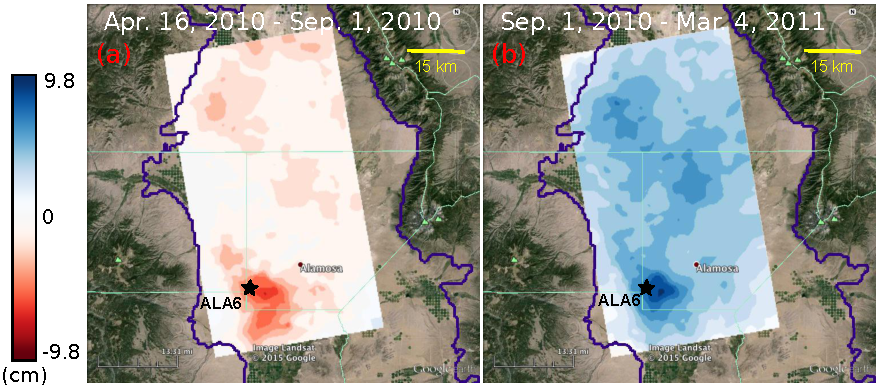
\includegraphics[width=0.9\textwidth]{Figures/slv_seasonal.pdf}
\caption{ (a) Seasonal subsidence signatures assocaited with summer pumping as inferred from an L-band ALOS InSAR data that spans April 16, 2010 and September 1, 2010. (b) Seasonal uplift signatures associated with winter recharge as inferred from an L-band ALOS InSAR data that spans September 01, 2010 and March 4, 2011.}
\label{fig:seasonal_def}
\end{figure}

\begin{figure}
\noindent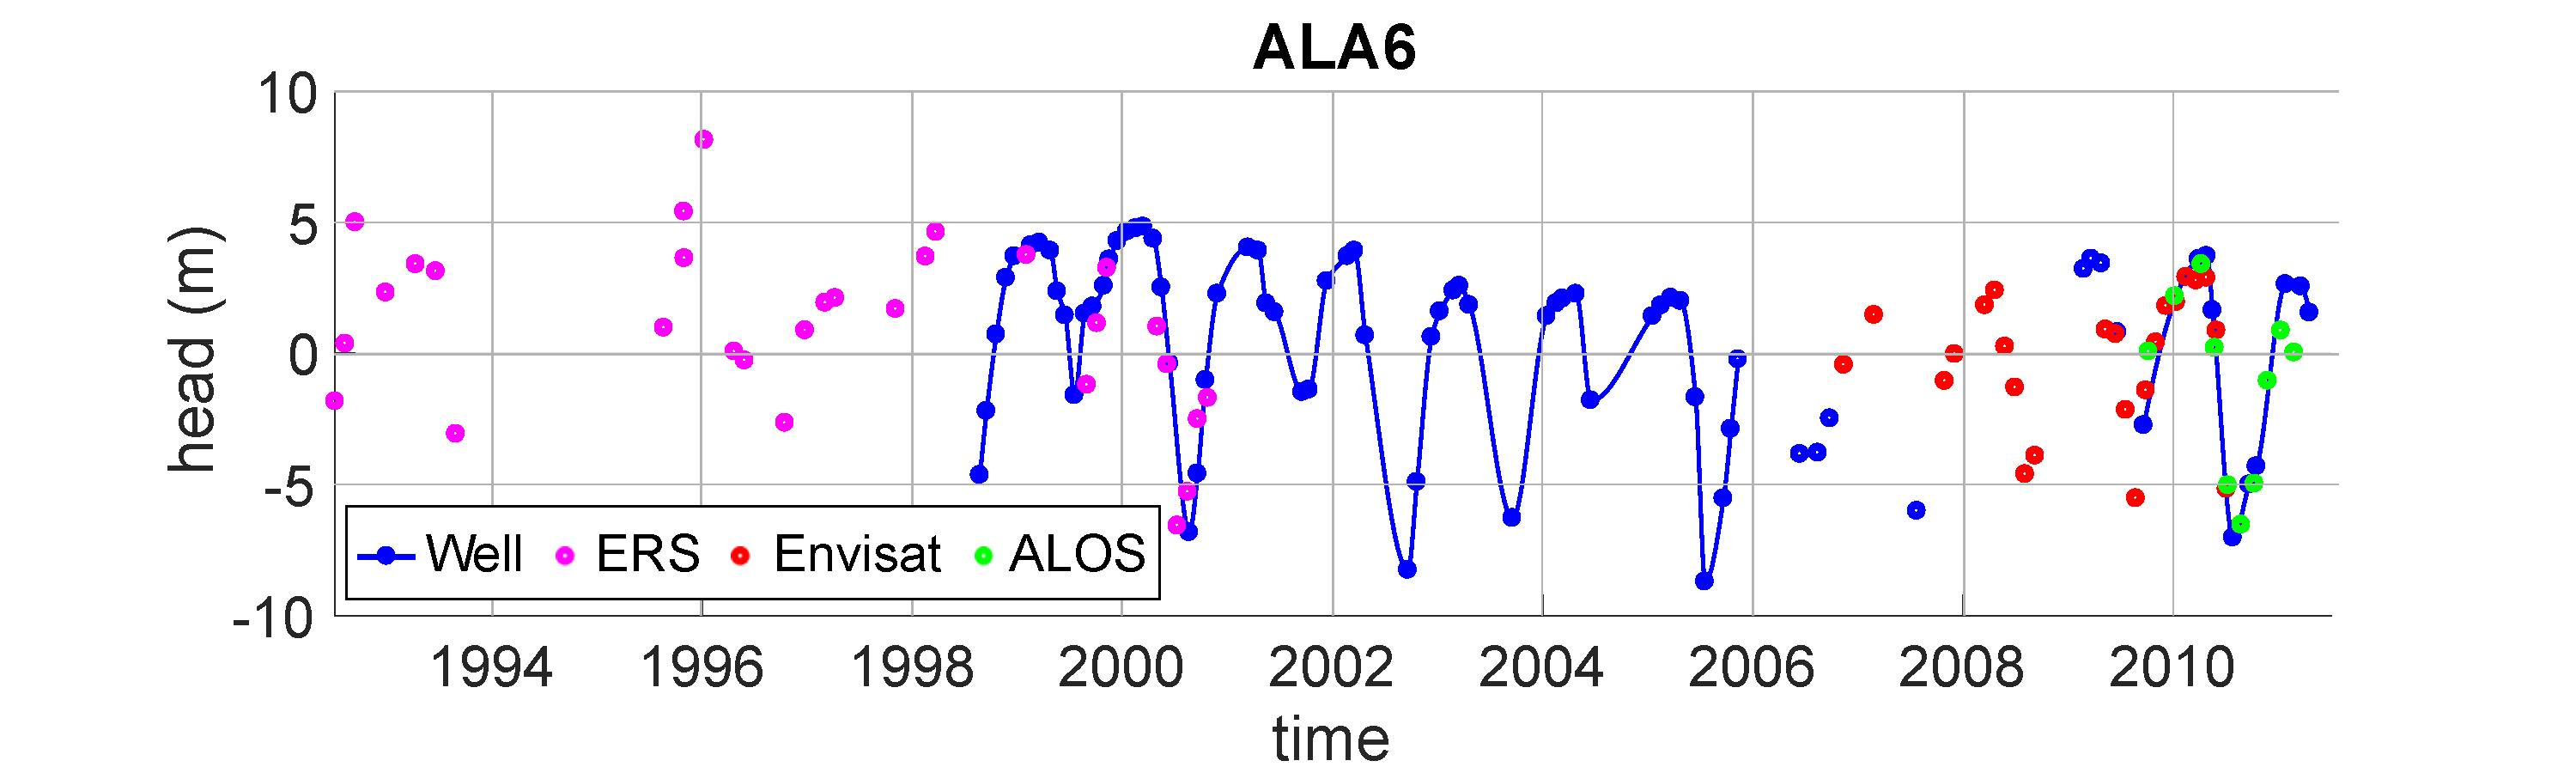
\includegraphics[width=0.9\textwidth]{Figures/ALA6.pdf}
\caption{Hydraulic head variations at the confined aquifer well ALA6 between 1992 and 2011 as measured from well data (in blue) and estimated from ERS-1/2 (in magenta), Envisat (in red) and ALOS PALSAR (in green) InSAR data. The same aquifer storage parameters ($S_{ke}$=0.00553 and $\tau$ = 6 days) were used to convert InSAR deformation time series of all three satellite missions to head. Using the interpolated well data as ground truth, the RMS error of the InSAR head estimates is 1.49 meters for the ERS-1/2 data, 0.75 meters for the Envisat data, and 1.21 meters for the ALOS data.}
\label{fig:ALA6}
\end{figure}

\subsection{Joint inversion of coupled geomechanics and subsurface flow}
In this section we describe our preliminary work on the poroelasticity inverse problem of inferring subsurface permeability from surface deformation and well data. Inference of subsurface permeability fields is commonly addressed through
subsurface flow inverse problems; some representative references include \citep{Carrera1986a,Carrera1986b,Carrera1986c,McLaughlin1996,Bohling2010,Cardiff2011,Cardiff2012,Berg2015,Yoon2017}. 
However characterization of the spatial variability of subsurface properties is limited because only point measurements of the parameters and the observed response are considered. Hydrogeophysical inversion includes additional and spatially distributed geophysical measurements to try to reduce this
uncertainty [70]. Our recent work [86] shows that the incorporation of time-series surface deformation data into a poroelastic model can significantly improve the characterization of reservoir permeability. A review of several case studies that have successfully used time series surface deformation measurements
to constrain reservoir properties can be found in [75], and a mathematical analysis of the coupled geomechanics/subsurface flow inverse problem is presented in [88]. Because we are inverting for parameter fields, the (discretized) inverse problem is very large scale, and computing the Bayesian solution presents formidable challenges. These are described next.

\subsection{Bio}
The PI and co-PI's bring together an interdisciplinary skill set modeling porous flow at different scales and have a history of collaboration and joint graduate student supervision \cite{Ghanbarzadeh2014,Ghanbarzadeh2015a,Ghanbarzadeh2015b,Ghanbarzadeh2017}.

\textbf{PI Hesse} has experience in modeling a broad range of porous media flows on the Darcy scale. He has made significant contributions to: reactive melt migration in viscously compacting porous media \cite{Hesse2003,Liang2010a,Liang2011b,Hesse2011,Schiemenz2011,Jordan2015,Arbogast2017,Jordan2018}, multi-phase flow in porous media \cite{Hesse2007,Hesse2008,Hesse2010,Golding2011,Sathaye2016b}, convection in porous media \cite{Riaz2006,Neufeld2010,MacMinn2012,Szulczewski2013a,Sathaye2014,Woods2015} and reactive flow in porous media \cite{Prigiobbe2012a,Prigiobbe2012b,Prigiobbe2013,Venkatraman2014,McNeece2016}. The PI also has experience developing numerical methods for Darcy-scale porous media flows \cite{Li2005,Hesse2008b,Schiemenz2011,Hesse2012,Hesse2014,Arbogast2017}.

\textbf{Co-PI Chen} has been on the forefront of ...

\textbf{Co-PI Ghattas} has been on the forefront of ...


\section{Proposed study}
In this section we describe proposed research aimed at overcoming the challenges elucidated in the previous sections. These include scalable parallel adaptive mesh forward solvers (§3.1) for the poromechanics model, faster MCMC sampling for Bayesian inversion (§3.2), and end-to-end model reduction for optimization under uncertainty (§3.3). This section also describes two application testbeds for studying control and management of CO2 injection and induced seismicity (§3.4–§3.5).

\subsection{In-situ and Remote Sensing Data Products}
As the basis for developing the Decision Support System, we need to quantify all relevant terms of the water balance equation. Historical head measurements of the SLV aquifer system can be accessed from the San Luis Valley Well and Water-Level Database (http://www.prinmath.com/rgwcd/). The hydraulic head in confined aquifers will be estimated using InSAR data shown in Figure \ref{fig:insar-mission} through calibration with local well measurements. The hydraulic head in unconfined aquifers will be quantified using relatively abundant shallow aquifer wells. To quantify other flux and storage terms in the water balance model, we will assimilate available satellite data products and models listed in Table \ref{tb:data} into the decision-support system. In addition, we will include the rain gauge data to calculate precipitation and USGS in-situ hydrologic data from surface water gauges to calculate the river runoff. Water levels in streams and lakes will be used to calculate the surface water storage change in rivers and lakes. We will also integrate forward looking predictions of snow melt and climate forecasts from National Operational Hydrologic Remote Sensing Center and NOAA Climate Prediction Center, which guide solution for the predictions of hydraulic head up to six months in advance.

\begin{figure}
\noindent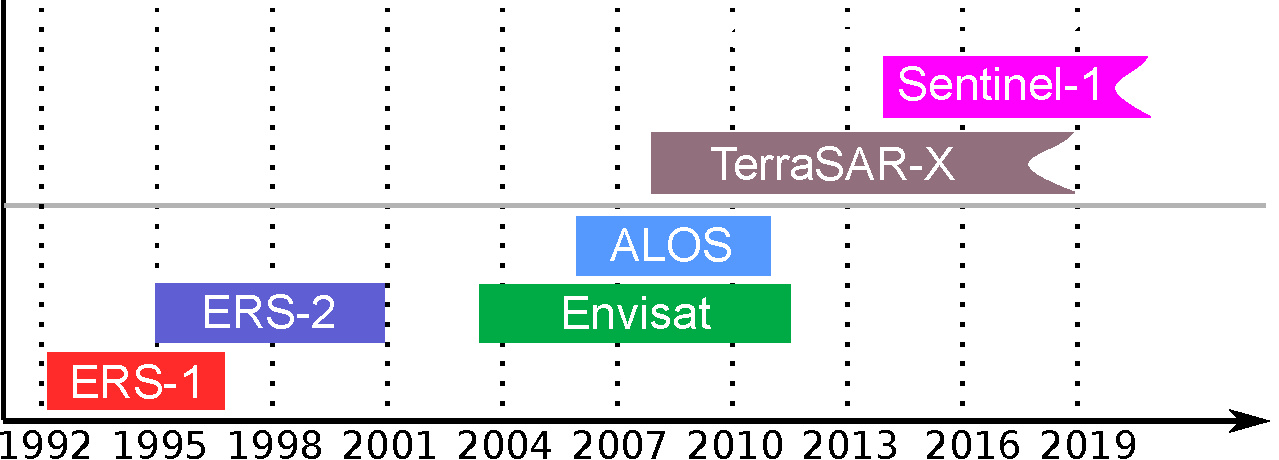
\includegraphics[width=0.7\textwidth]{Figures/InSARmissions.pdf}
\caption{Lifespans of recent SAR missions that we use to retrieve the historic head variation over the San Luis Valley, Colorado. The missions above the grey lines are currently in operations.}
\label{fig:insar-mission}
\end{figure}

\begin{table}
\caption{Satellite data and model products for quantifying key components in water cycle}
\centering
\begin{tabular}{c c c c }
\hline\hline
Satellite/Model & Start & End  & Product \\[0.5ex]
\hline
GRACE & 2002 & 2017 & Total Water Storage Change \\
GRACE-FO & 2018 & present & Total Water Storage Change \\
GPM & 2014 & present & Rainfall \\
SMAP & 2015& present & Surface Soil Moisture \\
AMSR-E & 2002 & 2011 & Surface Soil Moisture, Snow Water Equivalent \\
NLDAS & 1979 & present & Evapotranspiration, Root Zone Soil Moisture \\[1.0 ex]
\hline
\end{tabular}
\label{tb:data}
\end{table}

\subsection{Outstanding science questions}



\subsubsection{Numerical model development}\label{sec:num_darcy}

\subsection{Stochastic Newton MCMC for high-dimensional parameter
  space inversion} 
\label{sec:mcmc}

%The Bayesian inversion framework described above provides an
%expression for the posterior probability distribution of the inversion
%parameters.

The effectiveness of MCMC for sampling posterior pdfs
resulting from Bayesian inversion hinges on the
availability of good sample proposals, particularly for high
dimensional parameter spaces. A candidate for a sample should (1) have
a good chance of being accepted in the sample chain, (2) be as
independent as possible from the last sample,
% chain point, 
and (3) be inexpensive to compute. Two strategies to achieve these
targets---the {\em stochastic Newton MCMC method} and a {\em reduced
  order model-based delayed acceptance approach}---will be further
developed under this proposal, and applied to the poromechanics
system.

The stochastic Newton MCMC method, developed by members of our team in
\citep{MartinWilcoxBursteddeEtAl12, Bui-ThanhGhattas12d,
  PetraMartinStadlerEtAl13}, uses local gradient and Hessian
information of the the negative log posterior to construct a
proposal given by a local Gaussian approximation of the
posterior distribution. Thus, the method exploits the structure of
the underlying posterior pdf, and, in particular, captures the
highly stretched contours of the posterior that are typical for
ill-posed inverse problems, in which the data inform the model
parameters very well in some directions in parameter space, and poorly
in others. However, straightforward application of the stochastic
Newton method
% to sample the posterior 
is workable in modest dimensions only. The basic difficulty is that
explicit construction of the Hessian entails solution of as many
forward problems as there are parameters, which is prohibitive for
large-scale problems. We have overcome this difficulty by introducing
low-rank approximations of the data misfit component of the Hessian (see
\cite{MartinWilcoxBursteddeEtAl12,FlathWilcoxAkcelikEtAl11,
  Bui-ThanhBursteddeGhattasEtAl12_gbfinalist} for the finite
dimensional version of the algorithm, and
\cite{Bui-ThanhGhattasMartinEtAl13, Bui-ThanhGhattas12e} for the
infinite dimensional version), motivated by the compact nature of the
Hessian for many inverse problems (e.g., \cite{Bui-ThanhGhattas12a,
  Bui-ThanhGhattas12, FlathWilcoxAkcelikEtAl11,
  Bui-ThanhBursteddeGhattasEtAl12_gbfinalist,
  Bui-ThanhGhattasMartinEtAl13, MartinWilcoxBursteddeEtAl12,
  Bui-ThanhGhattas12f}). For example, for the global seismology
problem of inferring the distribution of earth elastic properties from
seismometer data \cite{Bui-ThanhGhattasMartinEtAl13,
  Bui-ThanhBursteddeGhattasEtAl12_gbfinalist}, we construct rank-1000
approximations of million-dimensional Hessians with essentially no
loss of information, giving us {\em three orders of magnitude
  effective dimensionality reduction}.

Despite the use of low-rank approximations, computing Hessian
information for every sample can be prohibitive, so we have
been examining strategies for Hessian reuse. In
\cite{PetraMartinStadlerEtAl13}, we compare several strategies, 
% with the target of minimizing the number of PDE solves per
% independent sample
namely (1) an independent sampler that uses the Gaussian approximation
at the MAP point as a proposal; (2) a modified stochastic Newton
method, which reuses the Hessian of the MAP point at every sample; and
(3) the ``classical'' stochastic Newton method, which recomputes the
Hessian at every sample point. We find that
for a prototype ice sheet dynamics problem, the modified stochastic Newton
method is the most efficient, measured in the number of PDE solves per
obtained independent sample.
% by a factor of 5--10 
%compared to the two other approaches for a problem with over 100
%parameters.
We will theoretically study these recycled Hessian variants
of the stochastic Newton MCMC method, and further develop them in the
context of the poroelastic inverse problem.
% We will also seek to 
% Our research will also target
%globalize stochastic Newton (i.e., make the method more robust when a
%local Gaussian approximation is not warranted) using trust region
%ideas, which are common in deterministic optimization.

The delayed acceptance MCMC method \cite{EfendievHouLuo06,ChristenFox05}
addresses the need to reduce the cost of MCMC for expensive forward
models. A trial step is first taken with an inexpensive model; only if
acceptance of this trial point is indicated, do we then evaluate the
acceptance criterion using the expensive PDE model to determine
whether the point may be added to the Markov chain. 
% for finding good sample point candidates by
% deploying an inexpensive model in a trial step to determine whether a
% candidate point may be accepted in the Markov chain. Only if,
% according to this first trial stage, a point in parameter space has a
% good chance of being accepted, the expensive PDE model is evaluated in
% a second stage and the MCMC acceptance test is employed.
The critical issue in this approach is the construction of an
inexpensive-to-evaluate but sufficiently accurate surrogate
model. Here, we will build on our experience in model reduction
methods (see \S\ref{sec:rom}) and construct a data-driven reduced
model by exploiting, once again, that the inverse problem solution
often lies in a low dimensional manifold \cite{CuiMarzoukWillcox14}.
The research question to be pursued is how to cover the parameter
space in order to obtain a reduced model that is accurate over the
posterior distribution; among others, we plan to adapt to the
poroelastic inverse problem the approach recently proposed in
\cite{CuiMartinMarzoukEtAl14}. Here, the relative influence of the
prior and the likelihood is characterized, and MCMC sampling is
performed only in the (effectively low-dimensional)
likelihood-informed directions, based again on structure-exploiting
low-rank Hessian approximations.


\section{Work plan} 



\subsection{Computational resources and data management}



\subsection{Individual contributions}

% \hspace{7mm}\textbf{Marc Hesse (PI):} Marc will coordinate the development of the Darcy-scale three-phase differentiation model. He will be the main thesis advisor of the geophysics graduate student developing the Darcy-scale computer model and co-advisor of the engineering graduate student developing the pore-scale computer model.  Marc will co-author conference abstracts and publications, and present results at conferences and invited talks. 

% \textbf{Ma{\v s}a Prodanovi{\'c} (Co-PI):} Ma{\v s}a will coordinate the development of the pore-scale three-phase textural equilibrium model. She will be the main thesis advisor of the engineering graduate student developing the pore-scale computer model and co-advisor of the geophysics graduate student developing the Darcy-scale computer model.  Ma{\v s}a will co-author conference abstracts and publications, and present results at conferences and invited talks. 

% \textbf{Engineering Graduate Student:} The student will initially run the two-phase model in texturally equilibrated pore networks. Later the student will extend the level-set method for texturally equilibrated pore networks to three phases. Finally he will use Lattice Boltzmann simulations on the computed networks to determine relative permeabilities. The student will be first author on papers resulting form this work and present his work at conferences.

% \textbf{Geophysics Graduate Student:} The student will extend the existing differentiation model to include three-phase flow and the enthalpy model to include silicate melting. Initial work will be in radial geometry, later the code will be extended to three dimensions. The student will be first author on papers resulting form this work and present his work at conferences.\\

\subsection{Schedule and milestones}
\noindent A tentative schedule of key milestones and accomplishments is presented in the following table:\\

\smallskip
%\begin{figure}[htb]
\centerline{\vbox{\def\bigstrut{\vphantom{$H^H_H$}}\def\0{\phantom{X }}
\newdimen\sem\sem=17pt
\def\active#1#2{\rlap{\hskip#1\sem\hbox to#2\sem{\rightarrowfill}}}
\offinterlineskip\halign{%
\bigstrut\hfil#\hfil\ &#\leaders\hbox to 1em{\hss$\cdot$\hss}\hfil\ &#&\vrule#&\vrule#\cr
%\omit\rlap{{\large\bf Table 1.  Timeline of proposed Work}}\cr
&\omit\hfil&\hfil Year 1\hfil&\hfil Year 2\hfil&\hfil Year 3\hfil\cr
&\omit\hfil Activity\hskip 140pt&\ Fa Sp Su\ &\ Fa Sp Su\ &\ Fa Sp Su\ \cr
\omit&\omit\phantom{:}&&&\cr
\noalign{\hrule}
\omit&\omit\phantom{.}&&&\cr
\noalign{\hrule}
\omit&\omit\phantom{:}&&&\cr
GEO & Development of three-phase Darcy model                 &\active{0}{2}&&\cr
GEO & Development of enthalpy method                         &\active{1}{2}&&\cr
GEO & Implementation of Darcy model in spherical symmetry    &\active{2}{3}&&\cr
GEO & Study planetesimal differentiation \& evolution        &\active{4}{5}&&\cr
GEO & Implementation of Darcy model three-dimensions         &\active{5}{4}&&\cr
ENG & Run two-phase flow in equilibrated pore networks       &\active{0}{3}&&\cr
ENG & Development three-phase textural eqbm model (2D)       &\active{1}{3}&&\cr
ENG & Development three-phase textural eqbm model (3D)       &\active{4}{5}&&\cr
ENG & Develop regime diagram for melt connectivity           &\active{6}{2}&&\cr
ENG & Relative permeability from LBM                         &\active{7}{2}&&\cr
}}}
%\end{figure}

\noindent Here GEO and ENG indicate task performed and supervised by the Geophysics (PI) and Engineering (co-PI) groups, respectively.

\newpage
\addcontentsline{toc}{section}{6\hspace{2.5mm} References}
\bibliographystyle{unsrt}
\bibliography{mendeley_v2,insar,ccgo}

\addcontentsline{toc}{section}{7\hspace{2.5mm} Data management plan}

% \setcounter{section}{6}
%\section{Data management plan}

\end{document}
